\chapter{RESULTADOS E DISCUSSÃO}
\label{cap:resultados}

\section{Módulo Professor}


O módulo implementado foi o do Professor. Para utilizar os componentes (Aluno, Aula, Avaliação e Diário), o sistema exige autenticação do usuário (Figura \ref{fig:loginTela}). Caso ainda não possua \textit{login}, basta optar pela criação de um novo usuário como mostrado na Figura \ref{fig:index}. O cadastro de professor é uma funcionalidade do módulo e é demonstrado nas Figuras \ref{fig:cadastroTela}, \ref{fig:assistenteInicialPT1}, \ref{fig:assistenteInicialPT2} e \ref{fig:assistenteInicialPT3}. Após terminar seu cadastro pessoal, o professor cria seu primeiro diário, que será demostrado posteriormente. Todas figuras aqui apresentadas, simulam o cadastro do professor fictício nomeado "Mallú Eduarda".

Finalizando esse processo, a página inicial é demostrada na Figura \ref{fig:telaInicio}. 

% Tela inicial da aplicação
\begin{figure}[!htb]
	\centering
	\caption{Tela inicial da aplicação} %legenda
	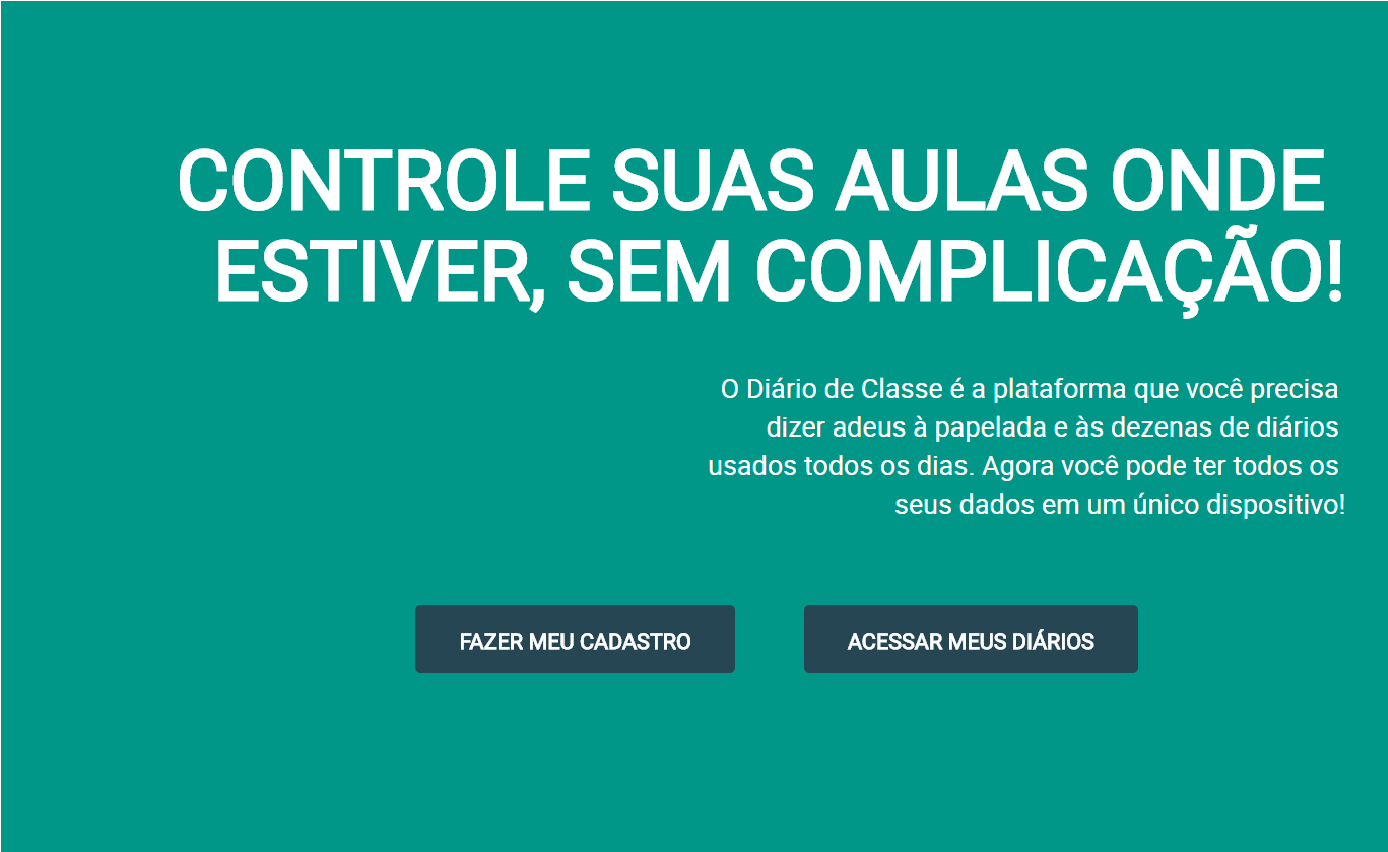
\includegraphics[scale=0.4]{index}\\  % o 0.9 indica 90% do tamanho original
	% pdfLaTeX aceita figuras no formato PNG, JPG ou PDF
	% figuras vetoriais podem ser exportadas para eps e depois convertidas para pdf usando epstopdf
	{\small } %Fonte da imagem
	\label{fig:index} %rotulo para refencia
\end{figure}

% Tela de cadastro
\begin{figure}[!htb]
	\centering
	\caption{Tela de cadastro de usuário} %legenda
	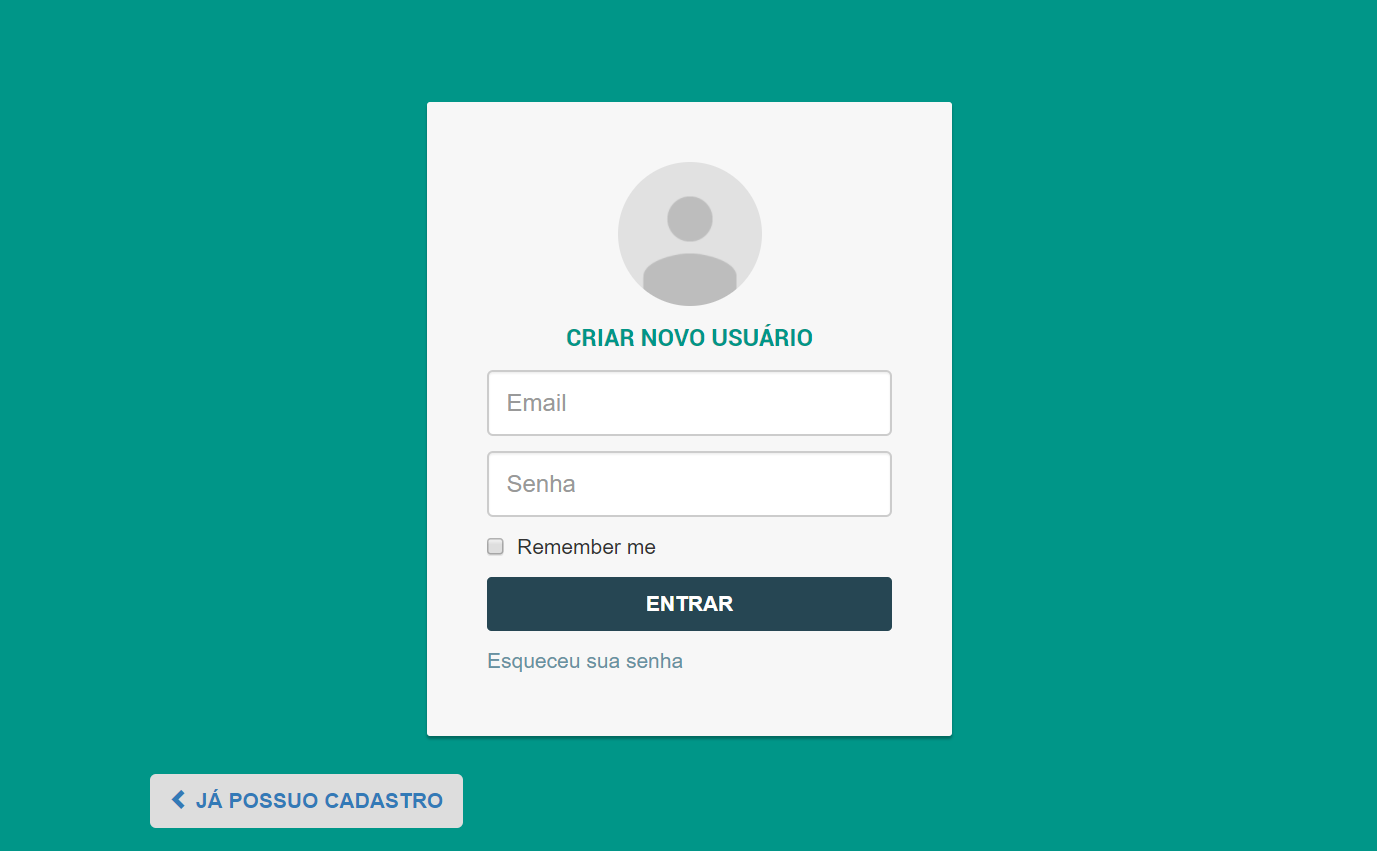
\includegraphics[scale=0.4]{cadastroTela}\\  % o 0.9 indica 90% do tamanho original
	% pdfLaTeX aceita figuras no formato PNG, JPG ou PDF
	% figuras vetoriais podem ser exportadas para eps e depois convertidas para pdf usando epstopdf
	{\small } %Fonte da imagem
	\label{fig:cadastroTela} %rotulo para refencia
\end{figure}


% Assistente Inicial pt1
\begin{figure}[!htb]
	\centering
	\caption{Assistente inicial: parte 1} %legenda
	
\includegraphics[scale=0.4]{assistenteInicialPT1}\\  % o 0.9 indica 90% do tamanho original
	% pdfLaTeX aceita figuras no formato PNG, JPG ou PDF
	% figuras vetoriais podem ser exportadas para eps e depois convertidas para pdf usando epstopdf
	{\small } %Fonte da imagem
	\label{fig:assistenteInicialPT1} %rotulo para refencia
\end{figure}

% Assistente Inicial pt2
\begin{figure}[!htb]
	\centering
	\caption{Assistente inicial: parte 2} %legenda
	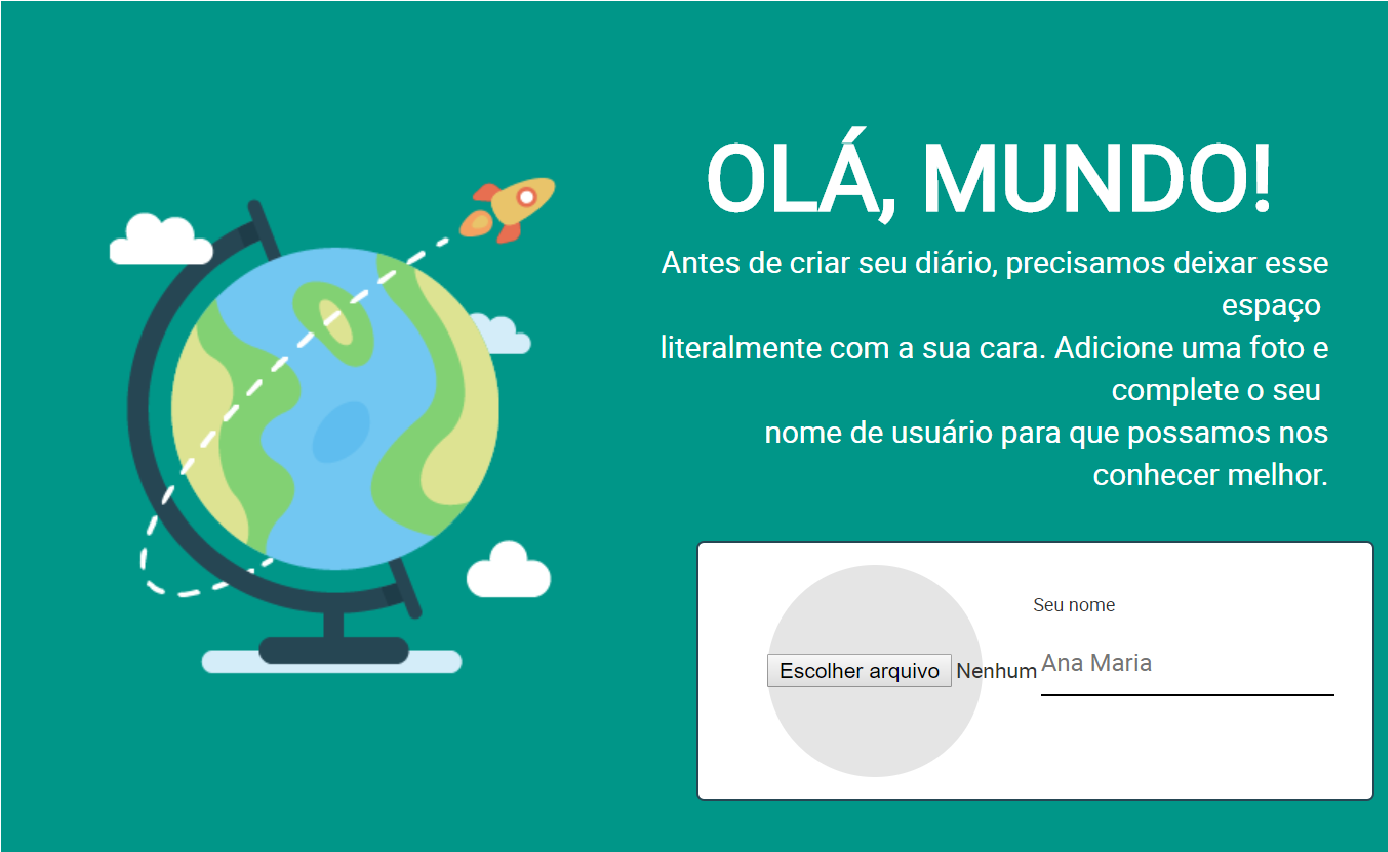
\includegraphics[scale=0.4]{assistenteInicialPT2}\\  % o 0.9 indica 90% do tamanho original
	% pdfLaTeX aceita figuras no formato PNG, JPG ou PDF
	% figuras vetoriais podem ser exportadas para eps e depois convertidas para pdf usando epstopdf
	{\small } %Fonte da imagem
	\label{fig:assistenteInicialPT2} %rotulo para refencia
\end{figure}

% Assistente Inicial pt3
\begin{figure}[!htb]
	\centering
	\caption{Assistente inicial: parte 3} %legenda
	
\includegraphics[scale=0.4]{assistenteInicialPT3}\\  % o 0.9 indica 90% do tamanho original
	% pdfLaTeX aceita figuras no formato PNG, JPG ou PDF
	% figuras vetoriais podem ser exportadas para eps e depois convertidas para pdf usando epstopdf
	{\small } %Fonte da imagem
	\label{fig:assistenteInicialPT3} %rotulo para refencia
\end{figure}

%Tela de login
\begin{figure}[!htb]
	\centering
	\caption{Tela de login} %legenda
	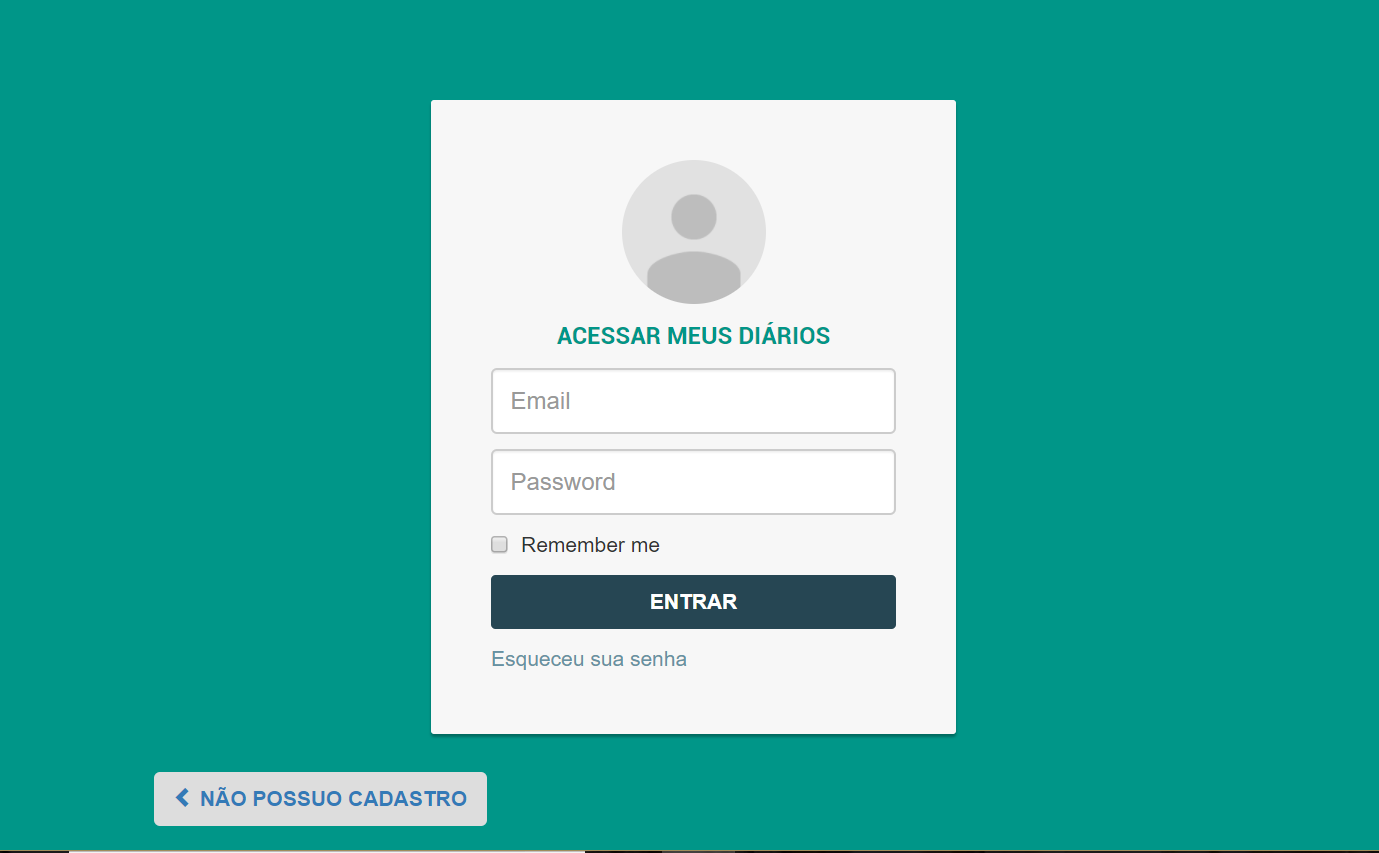
\includegraphics[scale=0.4]{loginTela}\\  % o 0.9 indica 90% do tamanho original
	% pdfLaTeX aceita figuras no formato PNG, JPG ou PDF
	% figuras vetoriais podem ser exportadas para eps e depois convertidas para pdf usando epstopdf
	{\small } %Fonte da imagem
	\label{fig:loginTela} %rotulo para refencia
\end{figure}

%pagina inicial professor
\begin{figure}[!htb]
	\centering
	\caption{Pagina inicial do professor} %legenda
	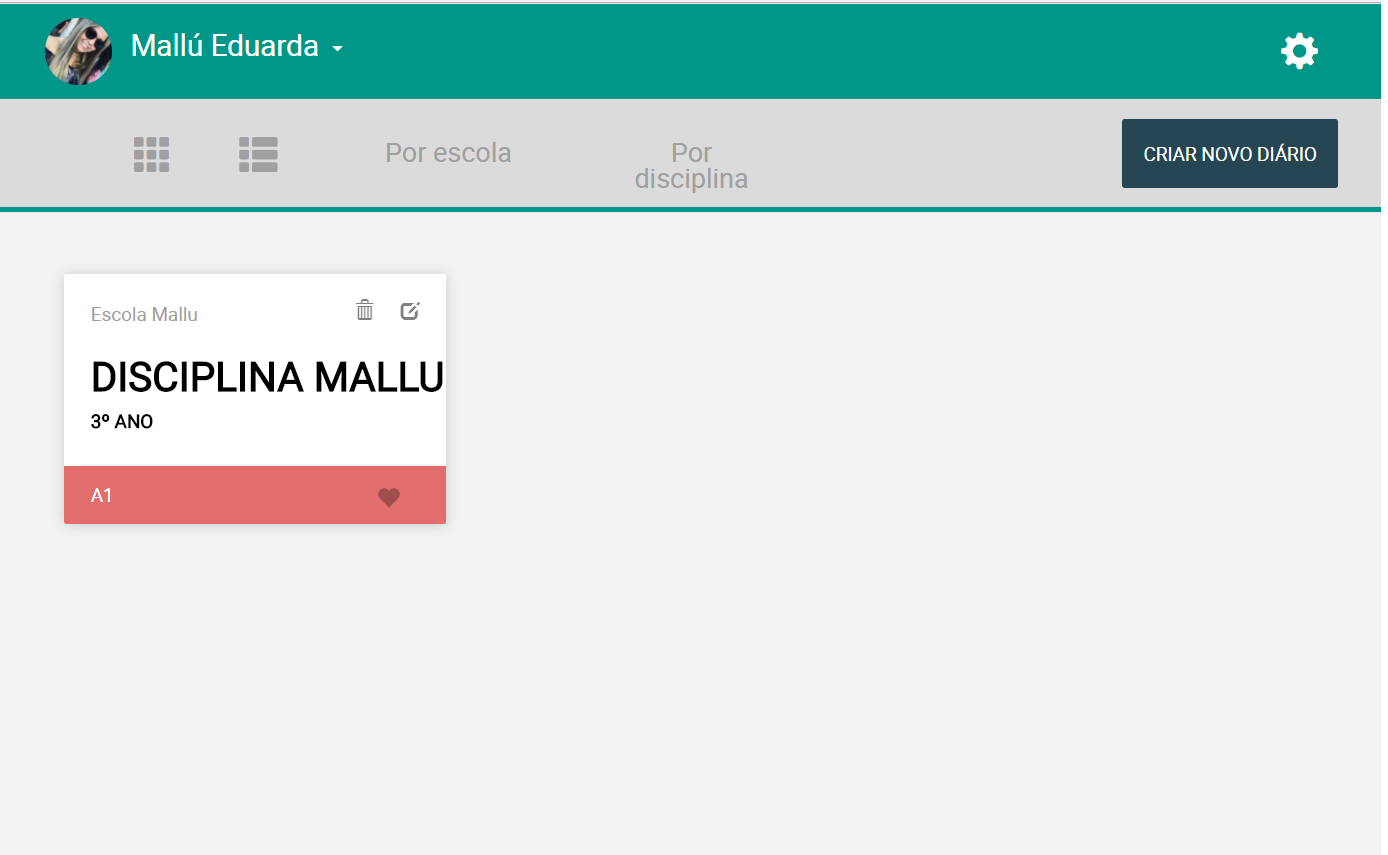
\includegraphics[scale=0.4]{telaInicio}\\  % o 0.9 indica 90% do tamanho original
	% pdfLaTeX aceita figuras no formato PNG, JPG ou PDF
	% figuras vetoriais podem ser exportadas para eps e depois convertidas para pdf usando epstopdf
	{\small } %Fonte da imagem
	\label{fig:telaInicio} %rotulo para refencia
\end{figure}


\section{Componentes}

\subsection{Diário}

Como componente principal, portador de todas as informações relevantes ao registro da prática pedagógica do professor, o diário de classe desempenha papel fundamental e único no módulo. As funcionalidades são: cadastrar, editar, excluir e visualizar diário. As mesmas, serão numeradas e explicadas posteriormente.

A função que carrega as informações e controla as requisições do usuário dentro de cada diário, é mostrada na figura \ref{fig:efetuaAcoes}. Cada clique em uma função é redirecionado para uma ação.


%controlador de ações do diário
\begin{figure}[!htb]
	\centering
	\caption{ Controlador de ações } %legenda
	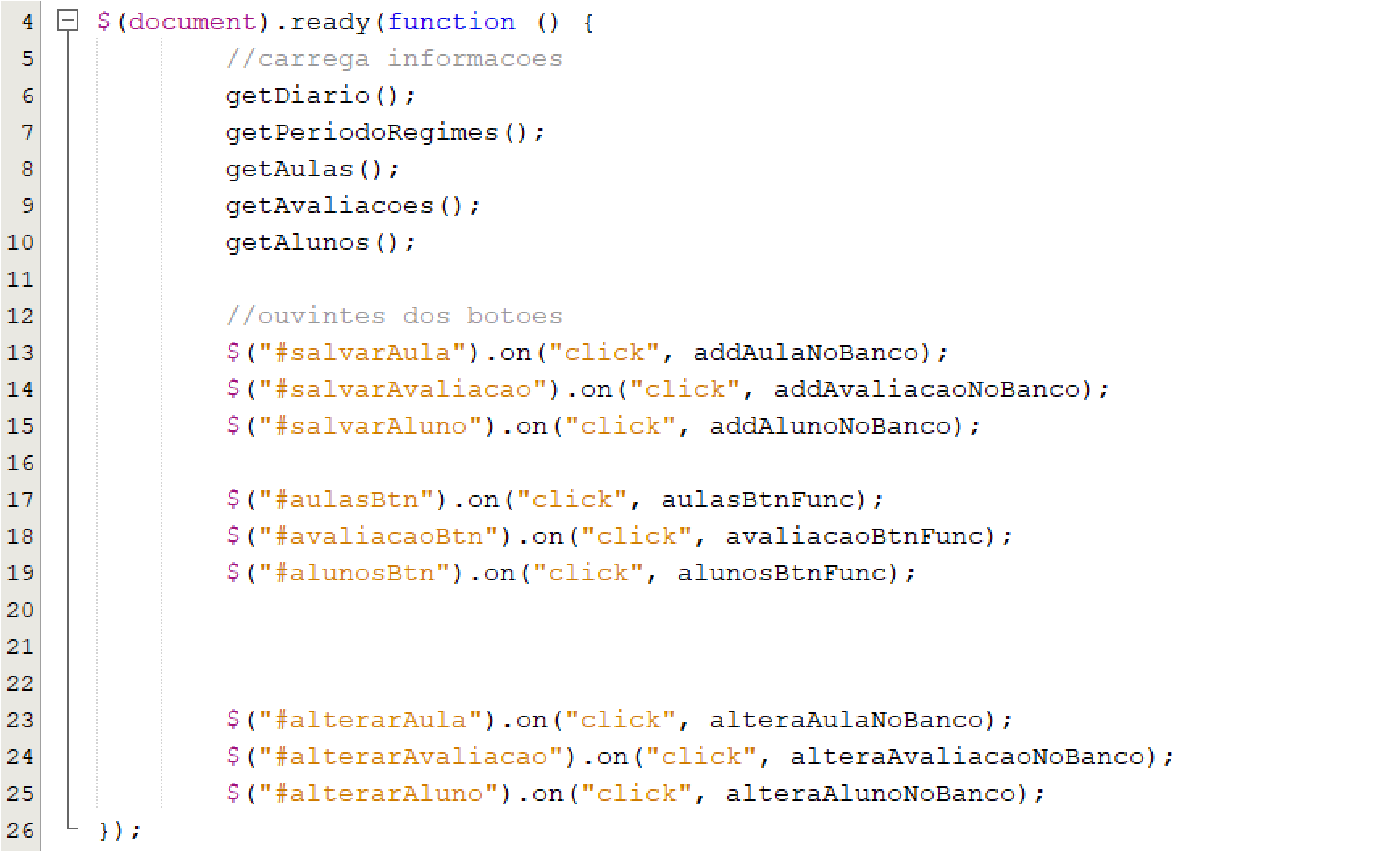
\includegraphics[scale=0.4]{efetuaAcoes}\\  % o 0.9 indica 90% do tamanho original
	% pdfLaTeX aceita figuras no formato PNG, JPG ou PDF
	% figuras vetoriais podem ser exportadas para eps e depois convertidas para pdf usando epstopdf
	{\small } %Fonte da imagem
	\label{fig:efetuaAcoes} %rotulo para refencia
\end{figure}


\begin{enumerate}
	\item Cadastrar:
	
	Na tela principal do usuário, existe o botão para cadastro de um novo diário. As informações solicitadas condizem com as presente no diário de papel, que é utilizado pelos professores. São solicitados o nome da escola, nome da disciplina, modalidade, série, identificação da turma e regime de aulas, como mostrado na Figura \ref{fig:cadastrarDiario}. Após a confirmação de preenchimento dos dados, eles são passados para próxima página, para completar o cadastro.
	
	 Nessa segunda parte, são solicitados dados referentes ao regime de aulas, definindo os períodos letivos, datas de início e fim para cada um, quantidade de aulas e o valor (em pontos) estipulado para o mesmo (Figura \ref{fig:cadastrarDiario2}). Essas informações são passadas ao controlador, que capta a "ação" pelo método POST, trata os dados necessários, cria o bean, executa no banco através do dao e redireciona para tela correspondente. Em caso de erro nesse processo, o usuário é informado e redirecionado para recadastrar os dados. Do contrário, a tela inicial com os diários cadastrados é retornada.
	
	
	
	%cadastrarDiario
	\begin{figure}[!htb]
		\centering
		\caption{Cadastrar Diário: parte 1} %legenda
		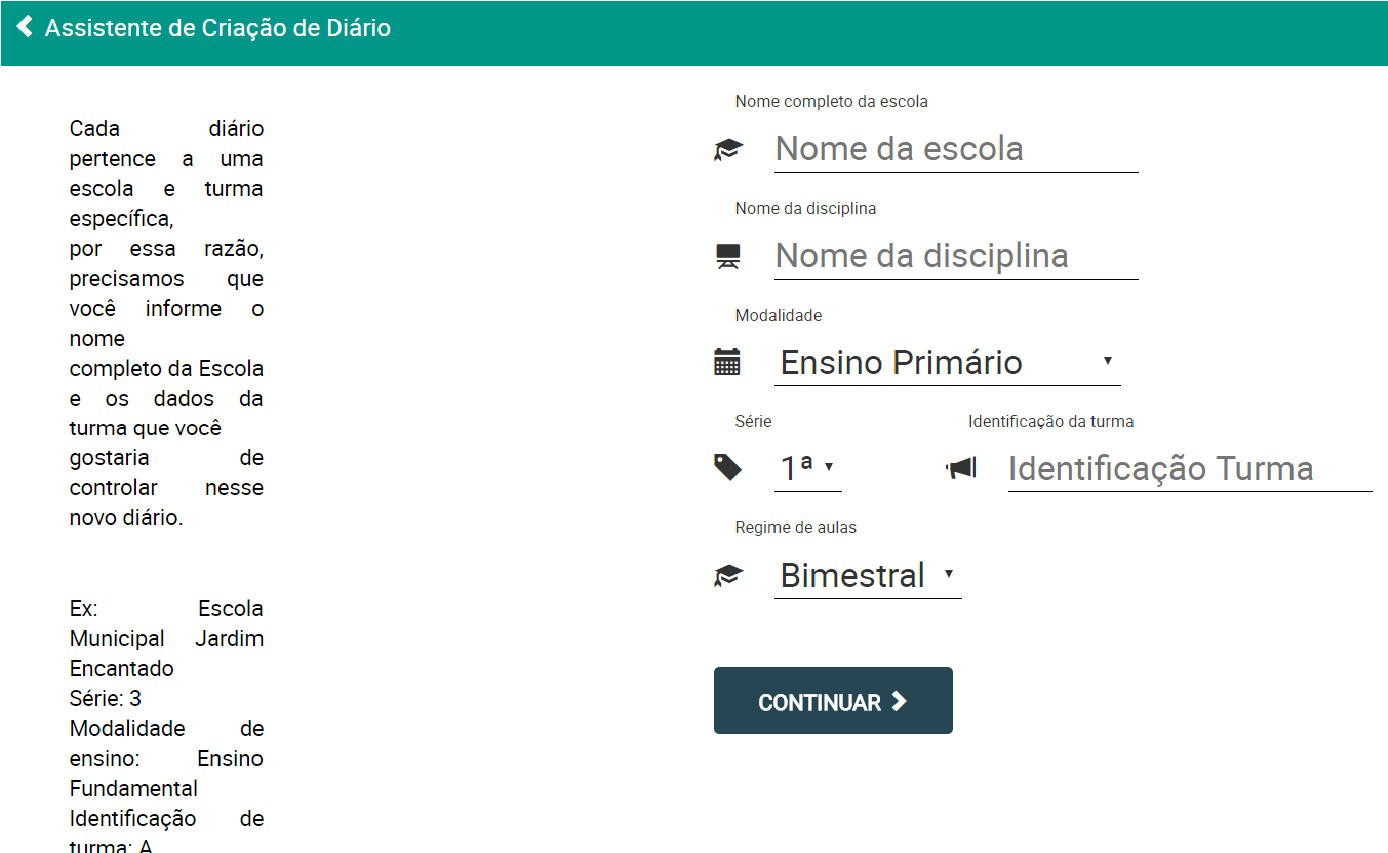
\includegraphics[scale=0.4]{cadastrarDiario}\\  % o 0.9 indica 90% do tamanho original
		% pdfLaTeX aceita figuras no formato PNG, JPG ou PDF
		% figuras vetoriais podem ser exportadas para eps e depois convertidas para pdf usando epstopdf
		{\small } %Fonte da imagem
		\label{fig:cadastrarDiario} %rotulo para refencia
	\end{figure}
	
	%cadastrarDiario2
	\begin{figure}[!htb]
		\centering
		\caption{Cadastrar Diário: parte 2} %legenda
		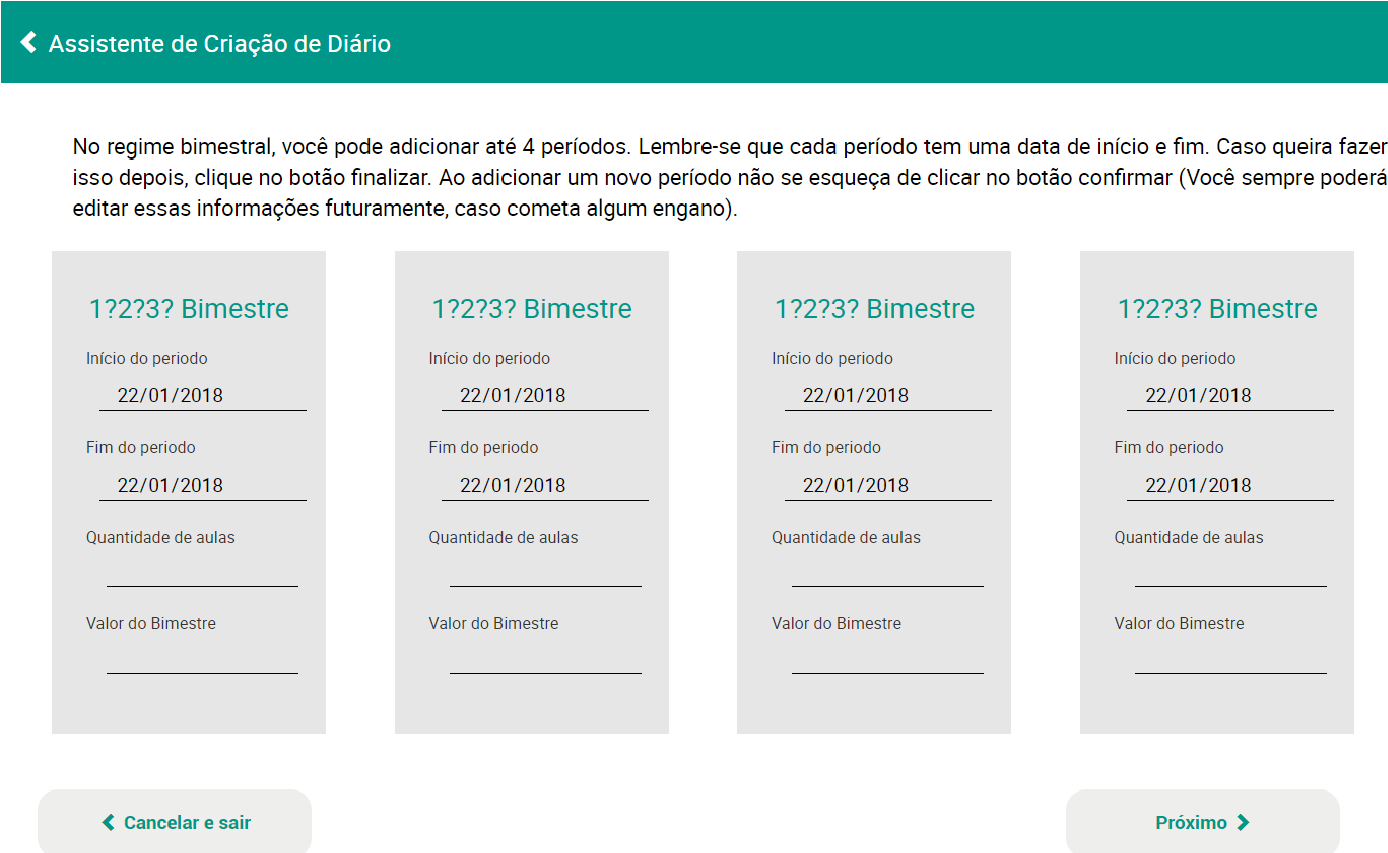
\includegraphics[scale=0.4]{cadastrarDiario2}\\  % o 0.9 indica 90% do tamanho original
		% pdfLaTeX aceita figuras no formato PNG, JPG ou PDF
		% figuras vetoriais podem ser exportadas para eps e depois convertidas para pdf usando epstopdf
		{\small } %Fonte da imagem
		\label{fig:cadastrarDiario2} %rotulo para refencia
	\end{figure}		
		

	
	
	
	%%%%%%%%%%%%%%%%%%%%%%	
	\item Editar:
	
	Ao optar pela edição do conteúdo, os dados são retornados para visão do usuário, advindos do banco de dados (Figuras \ref{fig:editarDiario} e  \ref{fig:editarDiario2}).
	
	%editarDiario
	\begin{figure}[!htb]
		\centering
		\caption{Editar Diário: parte 1} %legenda
		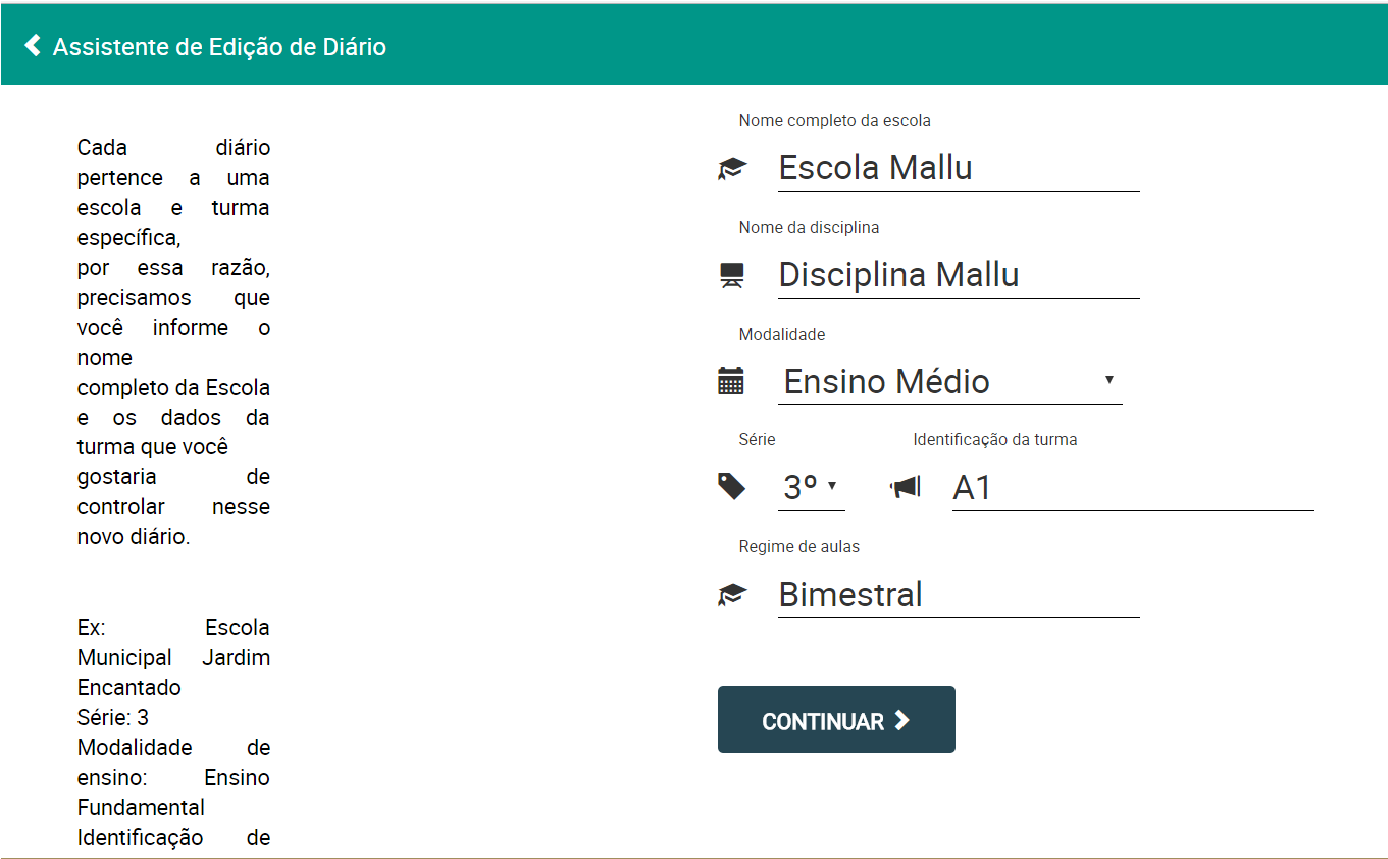
\includegraphics[scale=0.4]{editarDiario}\\  
		{\small } %Fonte da imagem
		\label{fig:editarDiario} %rotulo para refencia
	\end{figure}
	
		%editarDiario2
	\begin{figure}[!htb]
		\centering
		\caption{Editar Diário: parte 2} %legenda
		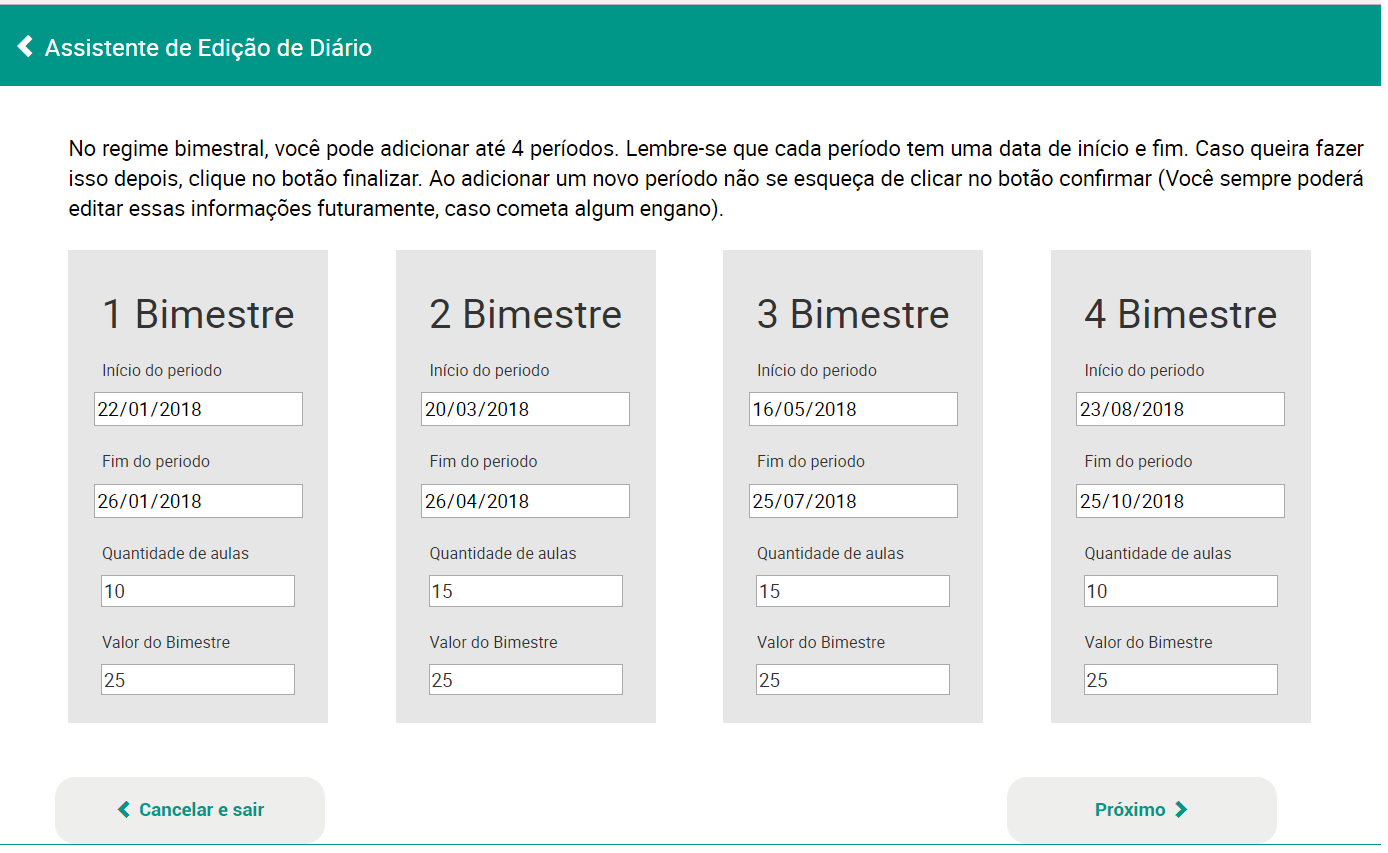
\includegraphics[scale=0.4]{editarDiario2}\\  
		{\small } %Fonte da imagem
		\label{fig:editarDiario2} %rotulo para refencia
	\end{figure}
	
	
	
	
	
	\item Excluir:
	
	Ao excluir um diário, as informações são apagadas da base de dados. 
	
	\item Visualizar:
	
	Os dados são dispostos para o usuário, em forma de acesso aos outros componentes. Pra complementar as informações do diário, podem ser adicionados alunos, aulas e avaliações ao diário. A figura 4.14 mostra o carregamento da pagina inicial do diário.
	
\end{enumerate}



\subsection{Aluno}

Os alunos de uma instituição, realizam seu cadastro por meio da secretaria. Esses dados são repassados diretamente para os professores, pela lista de chamada, através do diário de classe. O mesmo, possui acesso somente ao nome desses alunos.

Entretanto, nesse módulo, essas informações são inseridas manualmente como funcionalidade do sistema, pois não existe outro módulo senão o do professor. É possível cadastrar, editar, excluir, visualizar o boletim de cada aluno e visualizar os alunos.

%cadastrar aluno
\begin{figure}[!htb]
	\centering
	\caption{Cadastro de Aluno} %legenda
	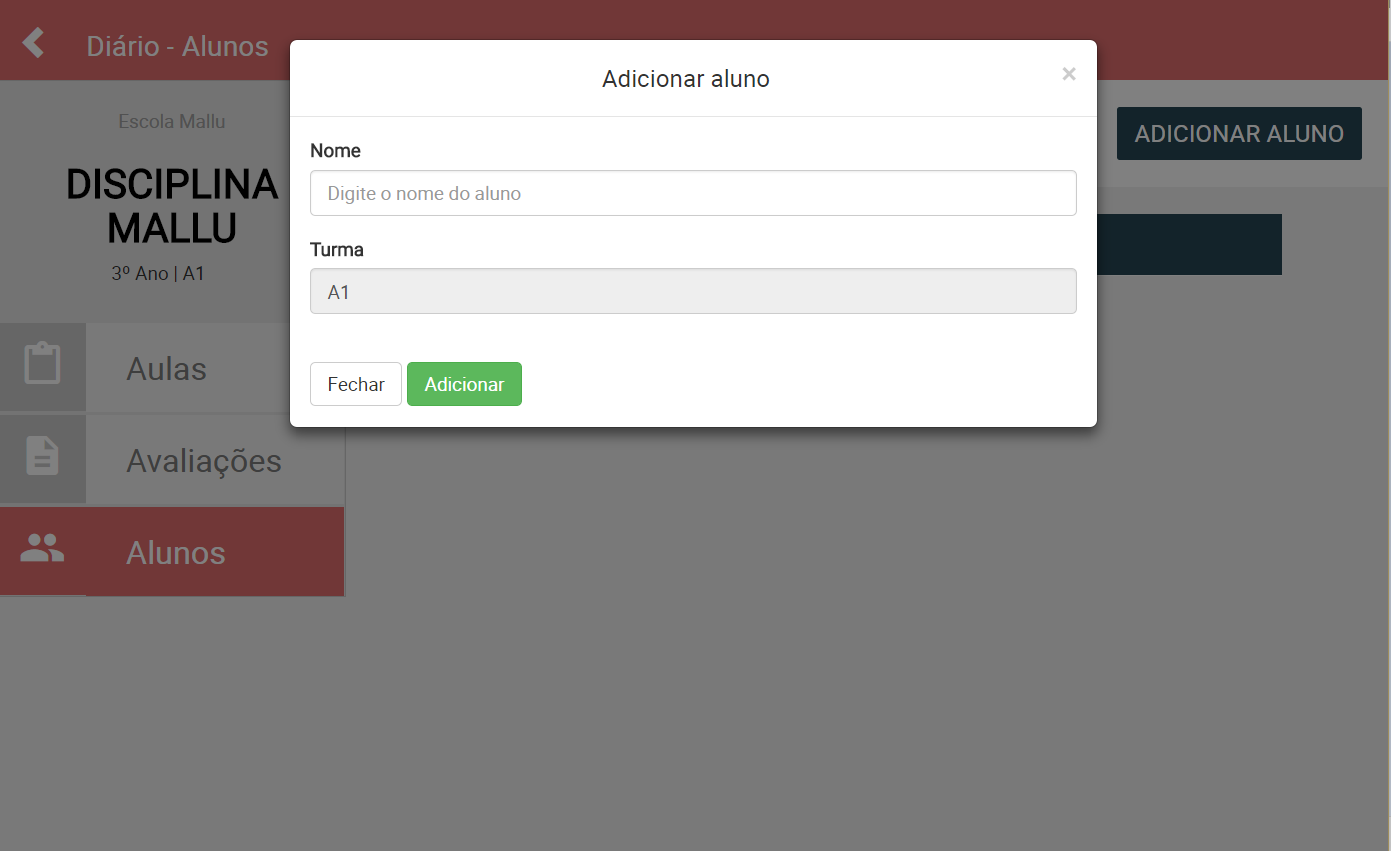
\includegraphics[scale=0.4]{cadastrarAluno}\\  % 
	{\small } %Fonte da imagem
	\label{fig:cadastrarAluno} %rotulo para refencia
\end{figure}

%visualizar aulas
\begin{figure}[!htb]
	\centering
	\caption{visualização dos Alunos } %legenda
	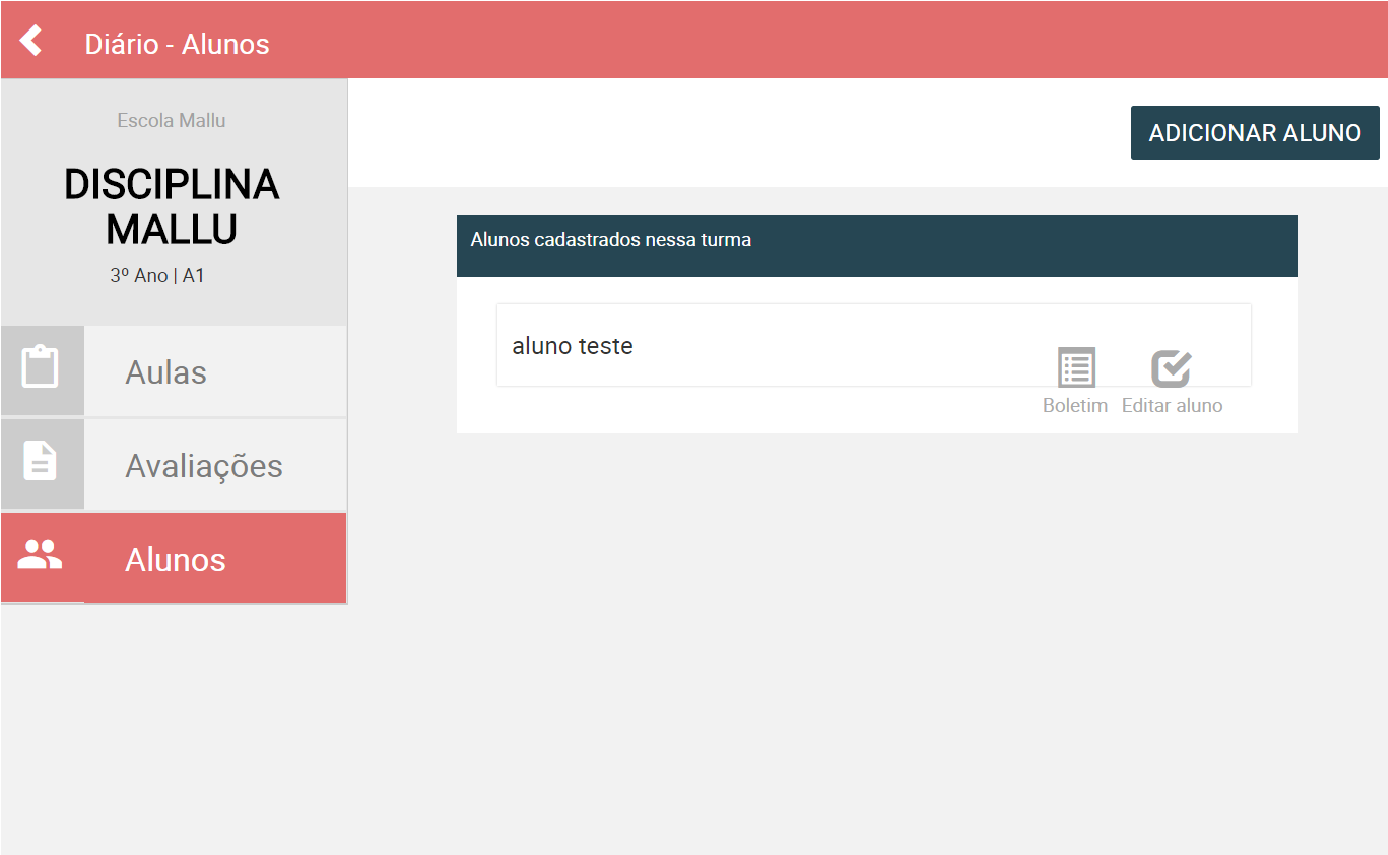
\includegraphics[scale=0.4]{visualizaAlunos}\\  % 
	{\small } %Fonte da imagem
	\label{visualizaAlunos} %rotulo para refencia
\end{figure}

%boletim
\begin{figure}[!htb]
	\centering
	\caption{Visualização do boletim do Aluno } %legenda
	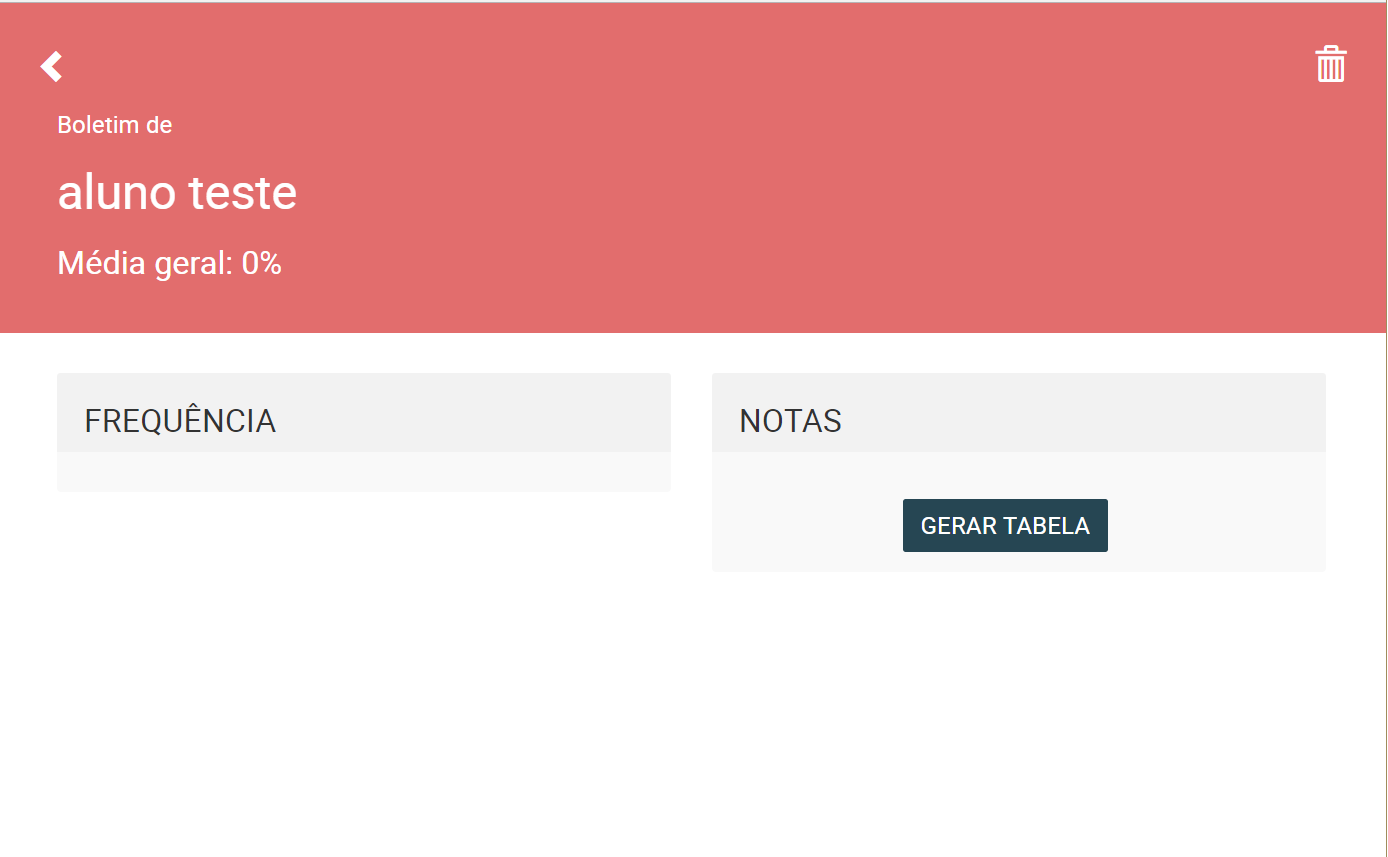
\includegraphics[scale=0.4]{boletimAluno}\\  % 
	{\small } %Fonte da imagem
	\label{boletimAluno} %rotulo para refencia
\end{figure}

\subsection{Aula}

Como parte das funções pedagógicas designadas ao professor, está o registro de aulas. Estas, devem possuir data e, uma descrição curta e objetiva sobre o conteúdo ministrado. Além de qualquer outra ocorrência de importância durante o período da aula.

Também é de responsabilidade do professor, efetuar a chamada, aluno por aluno, e registra-la com presença ou falta.

As funções de editar, cadastrar, excluir e visualizar são implementadas por meio de modais em java script que respondem a chamados da \textit{view}.


%cadastrar aula
\begin{figure}[!htb]
	\centering
	\caption{Cadastro de Aula} %legenda
	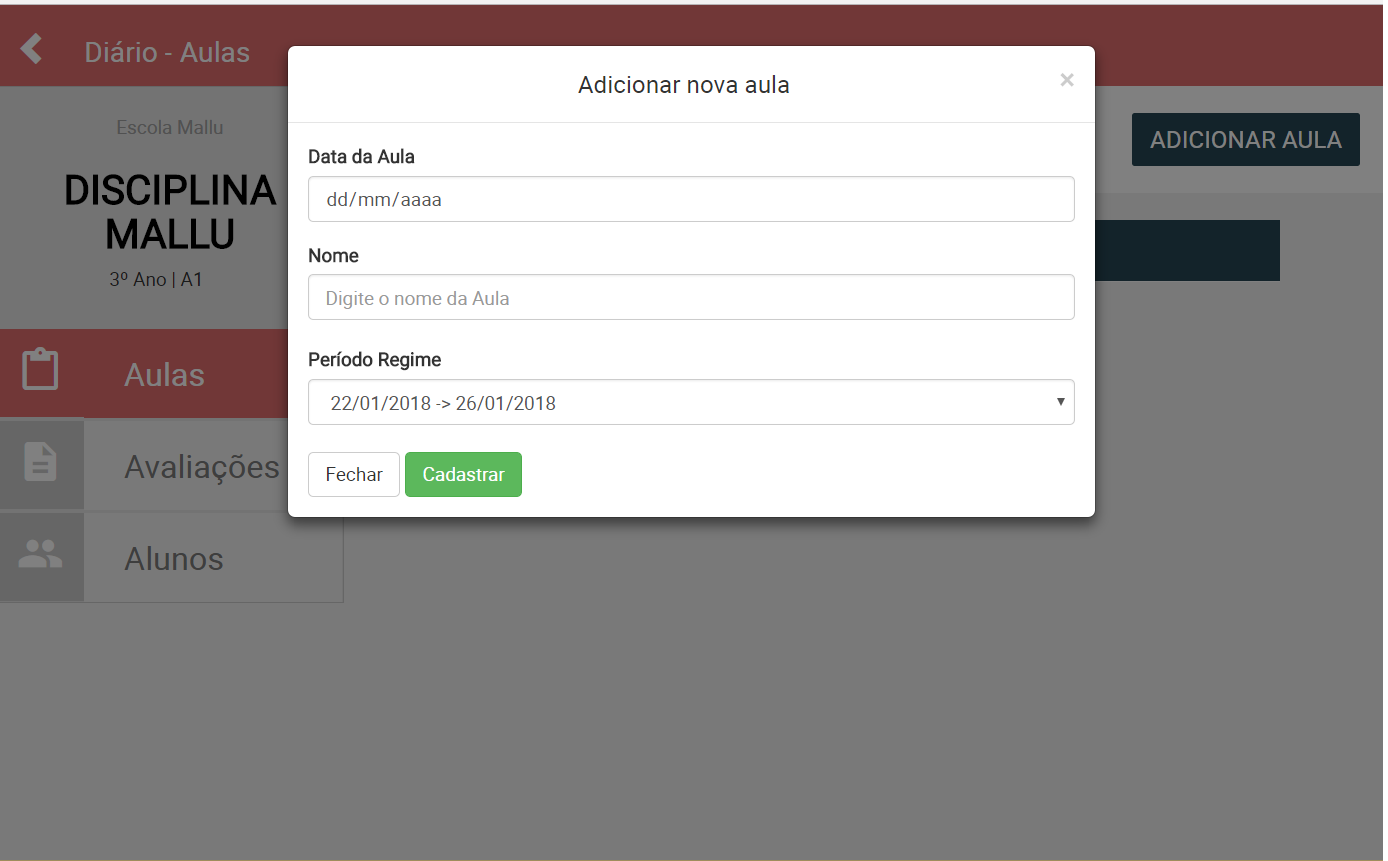
\includegraphics[scale=0.4]{cadastrarAula}\\  % o 
	{\small } %Fonte da imagem
	\label{fig:cadastrarAula} %rotulo para refencia
\end{figure}

%visualizar aulas
\begin{figure}[!htb]
	\centering
	\caption{Visualização das Aulas } %legenda
	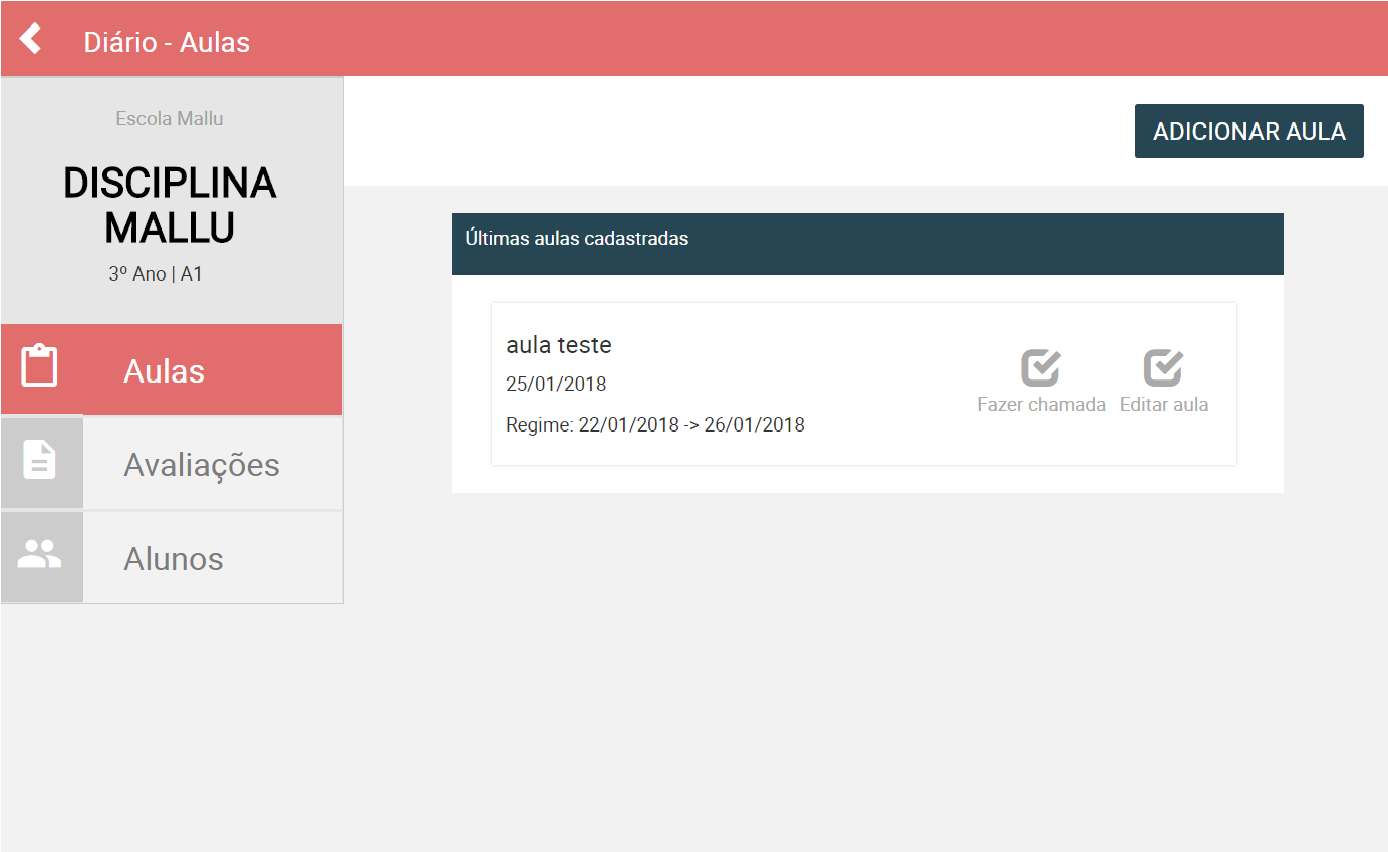
\includegraphics[scale=0.4]{visualizaAulas}\\  % 
	{\small } %Fonte da imagem
	\label{visualizaAulas} %rotulo para refencia
\end{figure}

%presença
\begin{figure}[!htb]
	\centering
	\caption{Listar presença dos Alunos na Aula } %legenda
	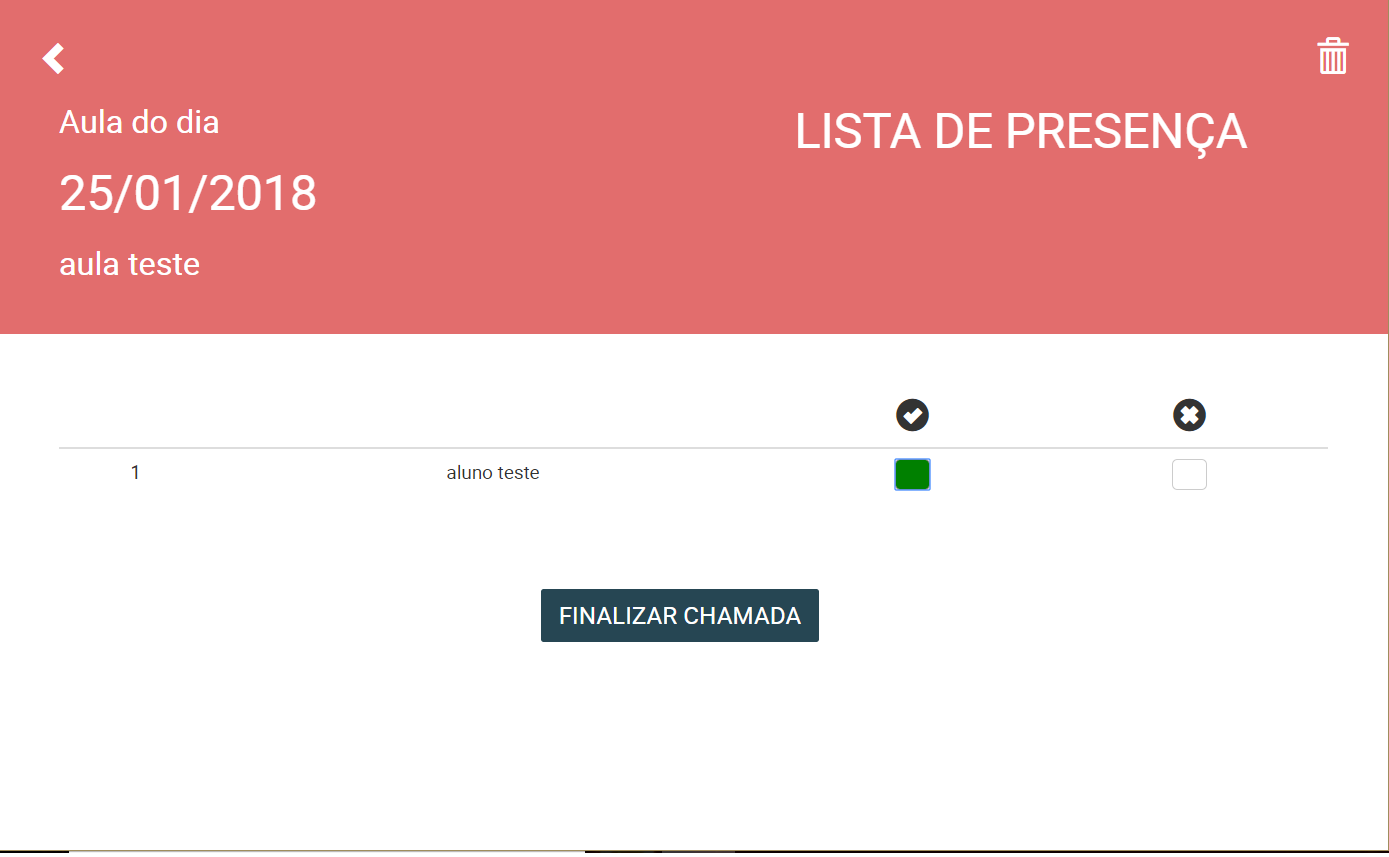
\includegraphics[scale=0.4]{listaPresenca}\\  % 
	{\small } %Fonte da imagem
	\label{listaPresenca} %rotulo para refencia
\end{figure}

\subsection{Avaliação}

Cada período letivo possui um valor. O somatório destes, corresponde ao total de cem pontos no ano letivo e é distribuído em avaliações no decorrer deste. Avaliações são métodos que tem por objetivo dar nota as atividades propostas aos alunos e devem ser registradas no diário pelo professor.

%cadastrar avaliação
\begin{figure}[!htb]
	\centering
	\caption{Cadastro de Avaliacao} %legenda
	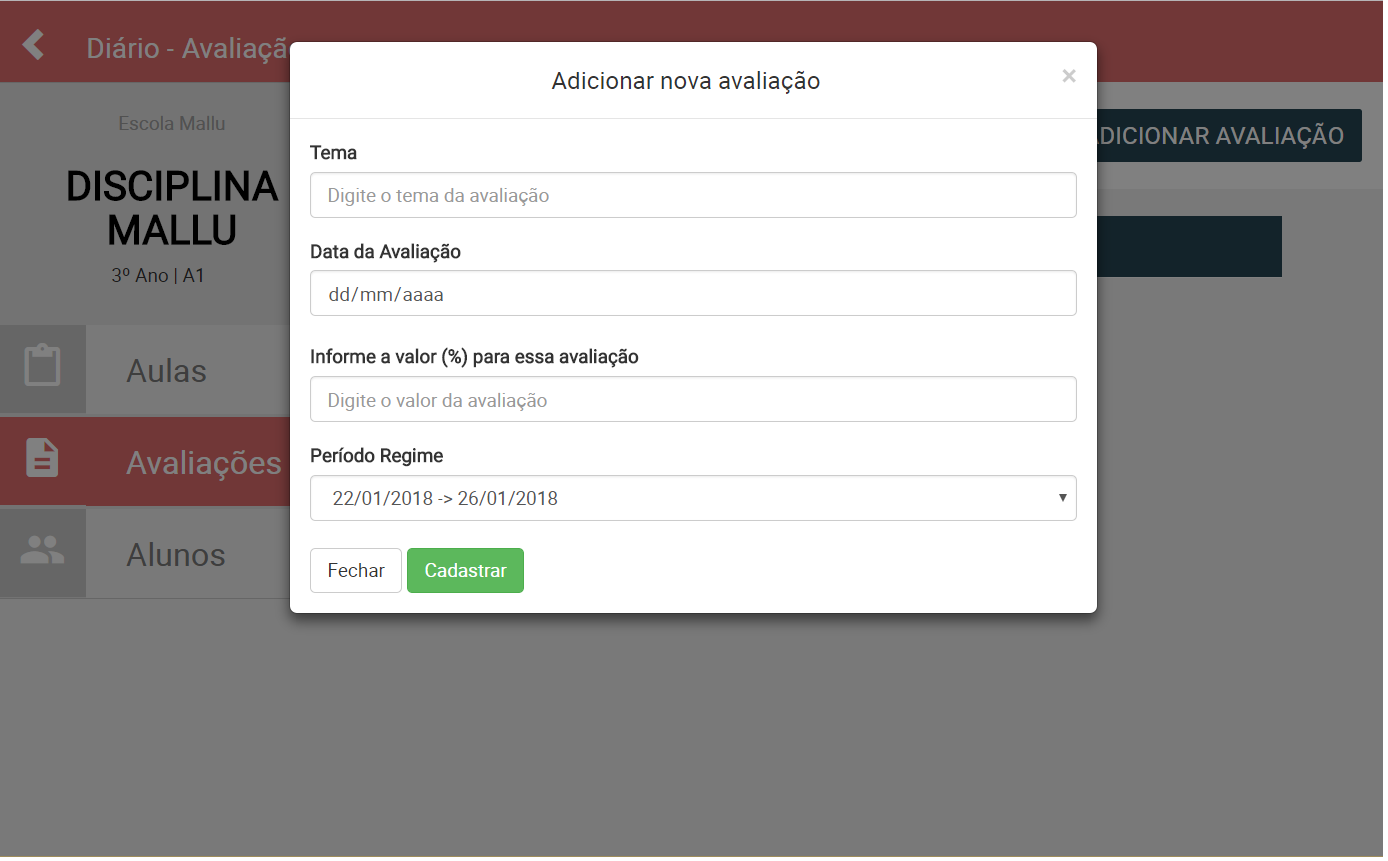
\includegraphics[scale=0.4]{cadastrarAvaliacao}\\ 
	{\small } %Fonte da imagem
	\label{fig:cadastrarAvaliacao} %rotulo para refencia
\end{figure}

%visualizar 
\begin{figure}[!htb]
	\centering
	\caption{Visualização das Avaliações } %legenda
	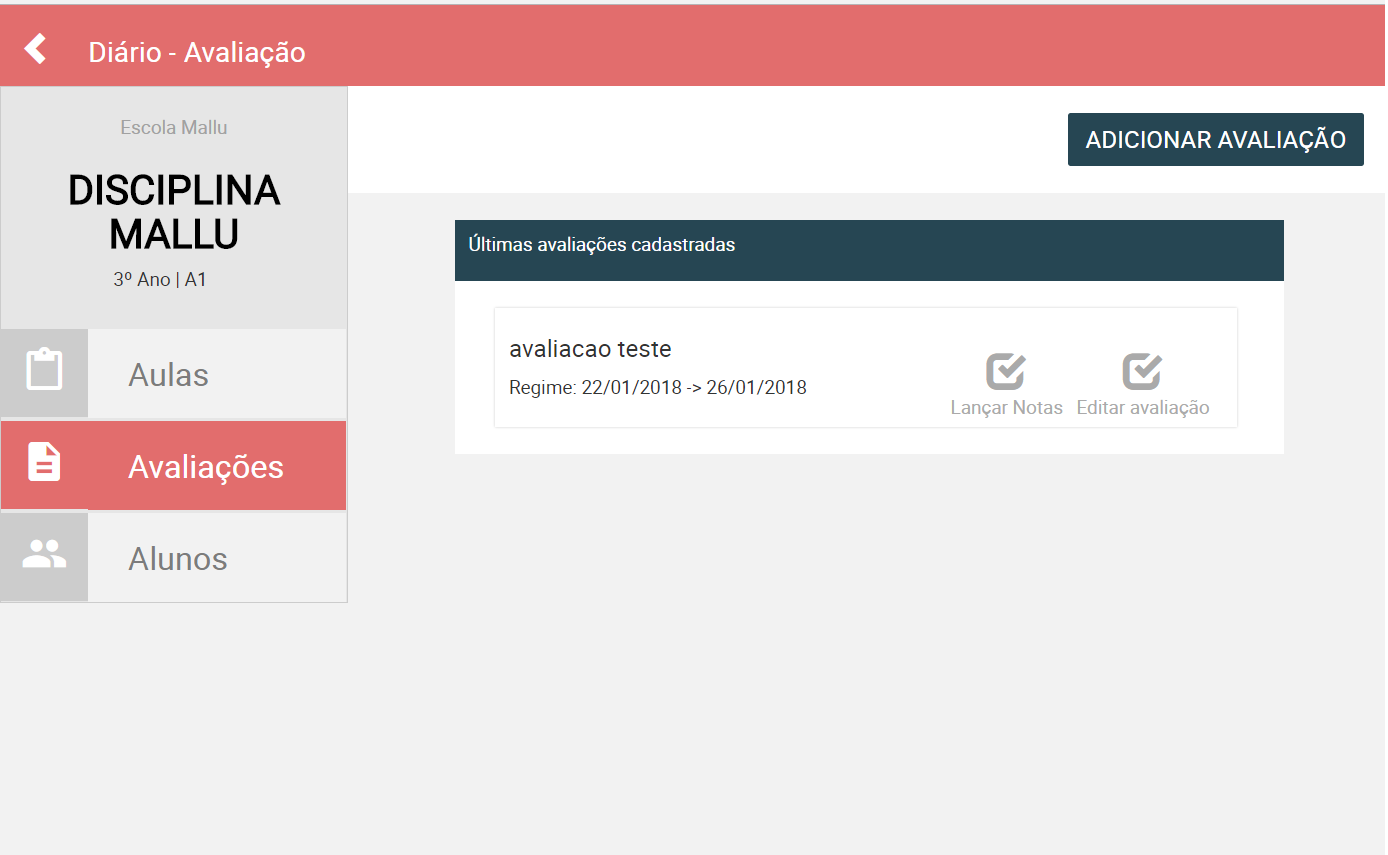
\includegraphics[scale=0.4]{visualizaAvaliacoes}\\  % 
	{\small } %Fonte da imagem
	\label{visualizaAvaliacoes} %rotulo para refencia
\end{figure}

%notas 
\begin{figure}[!htb]
	\centering
	\caption{Lançar nota de Avaliação } %legenda
	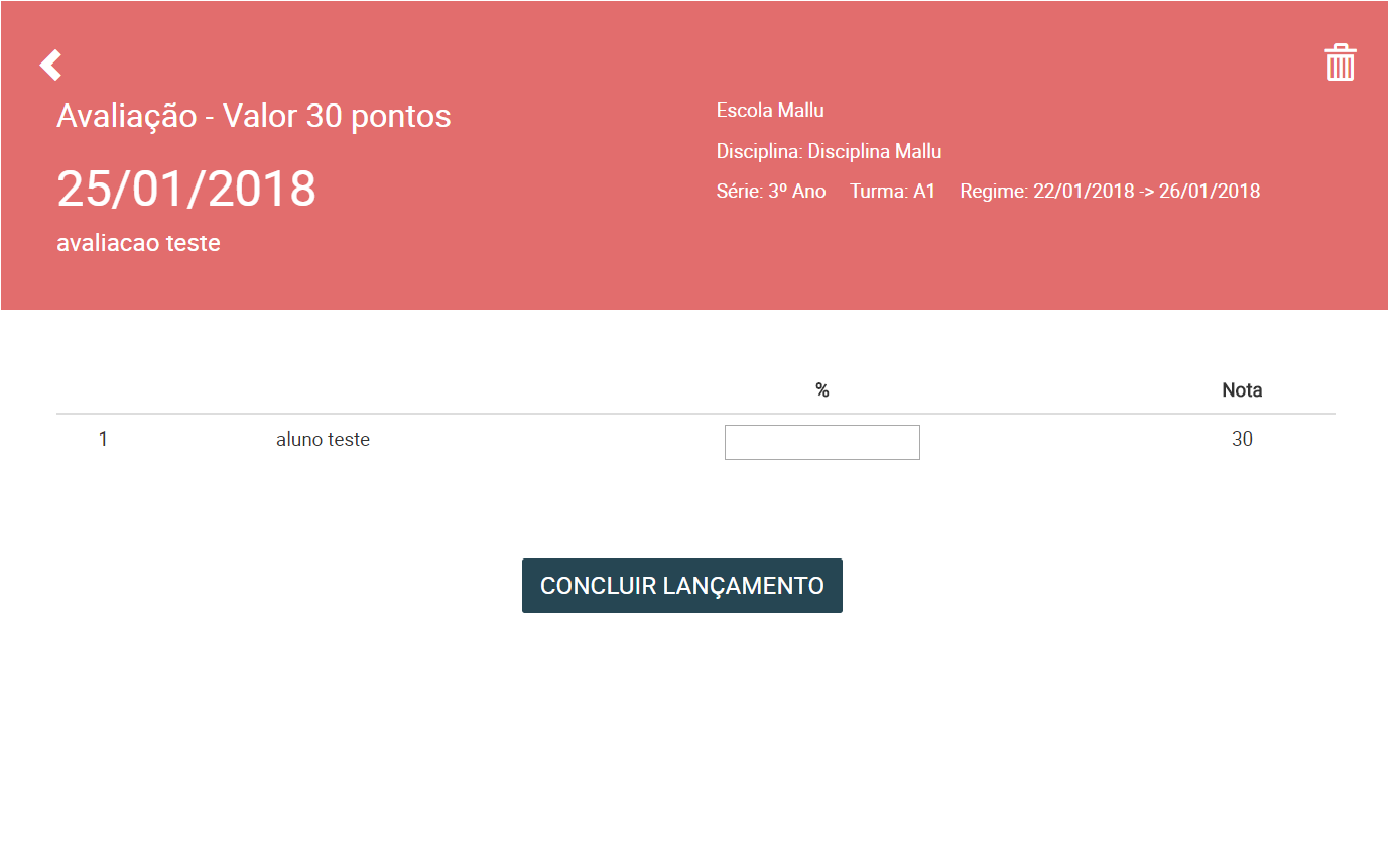
\includegraphics[scale=0.4]{notas}\\  % 
	{\small } %Fonte da imagem
	\label{notas} %rotulo para refencia
\end{figure}